\begin{figure*}[t]
\centering
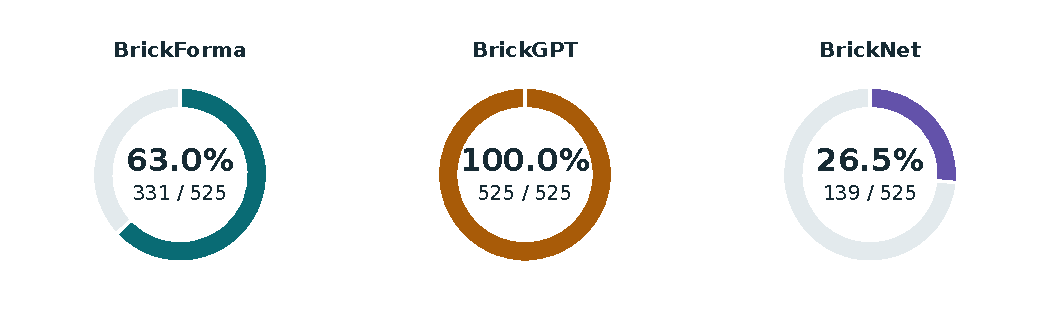
\includegraphics[width=\textwidth]{figures/comparison_20261117/01-zero-invalid.pdf}
\caption{Outputs with zero invalid placements on the 525 matched prompts. Colored arcs show outputs with $P_{\mathrm{inv}}=0$, and gray arcs show outputs with $P_{\mathrm{inv}}>0$. Each panel contains 525 outputs.}
\label{fig:comparison-zero-invalid}
\end{figure*}

\begin{figure*}[t]
\centering
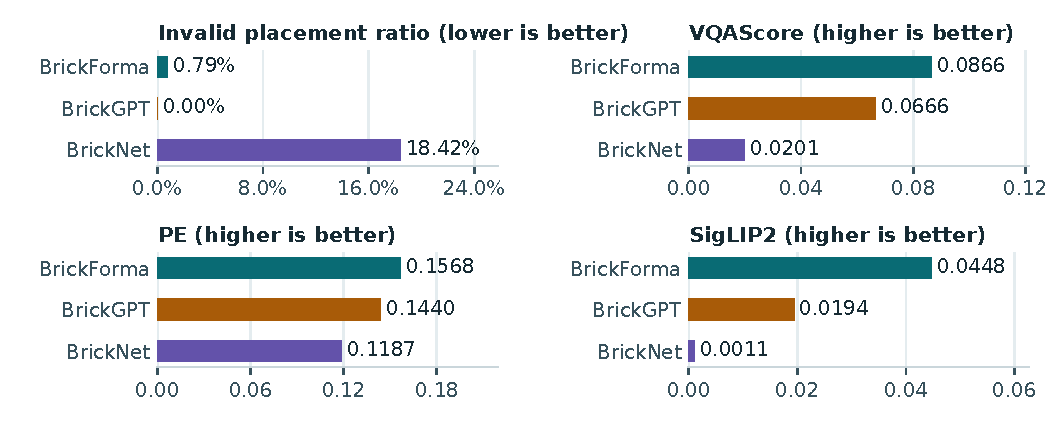
\includegraphics[width=\textwidth]{figures/comparison_20261117/02-means.pdf}
\caption{Mean scores on the 525 matched prompts. Each mean weights all prompts equally. The plotted values match Table~\ref{tab:main}.}
\label{fig:comparison-means}
\end{figure*}

\begin{figure*}[t]
\centering
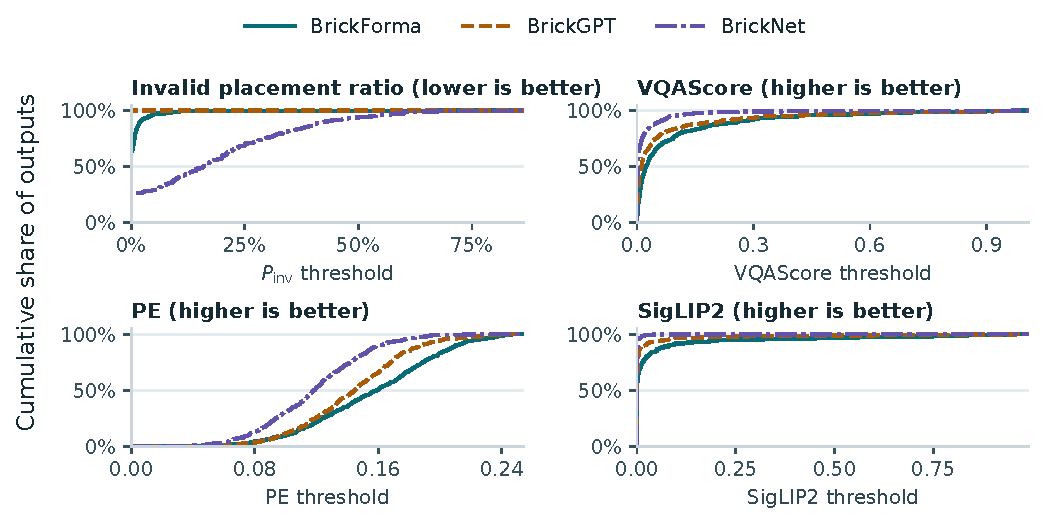
\includegraphics[width=\textwidth]{figures/comparison_20261117/03-distributions.pdf}
\caption{Empirical cumulative distributions of the four scores. Each curve gives the fraction of a system's 525 outputs that score at or below the threshold on the horizontal axis.}
\label{fig:comparison-distributions}
\end{figure*}

\begin{figure*}[t]
\centering
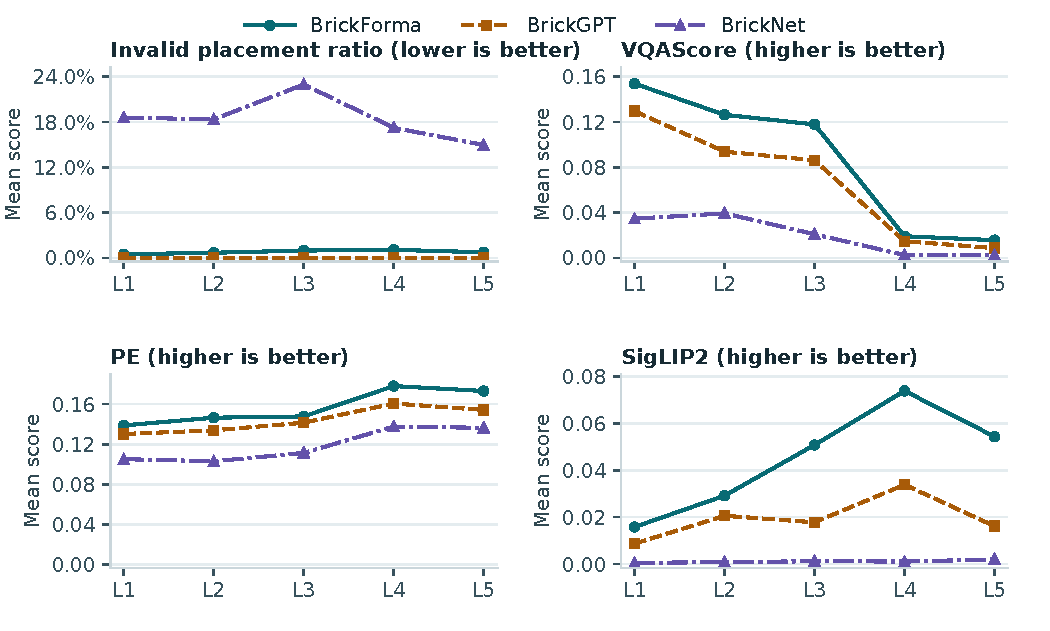
\includegraphics[width=\textwidth]{figures/comparison_20261117/04-by-level.pdf}
\caption{Mean scores from L1 to L5. Each point averages the 105 prompts shared by all three systems at that level (Table~\ref{tab:level-results}). From L3 to L4, VQAScore falls for all three systems, while PE rises.}
\label{fig:comparison-levels}
\end{figure*}
